Ce chapitre représente le point de départ de mon travail. Premièrement,
j'analyse et
je spécifie les besoins du projet. Ensuite, j'identifie les différents
acteurs. Et enfin, je
modélise le tout dans un diagramme des cas d’utilisation général qui
sera notre file conducteur
durant la prochaine phase.
\section{Périmètre du projet}
\subsection{Introduction à l'analyse}
Certes, la gestion des données en utilisant des solutions
Web ne date pas d'hier. Mais,
elle demeure une solution optimisant en terme de temps et de
productivité. Surtout,
dans un tel cas où les informations sont, à la fois, cruciales et
nombreuses. Ainsi, la solution proposée premièrement par la \textbf{DGCT} est
d'avoir une plateforme Web pour faciliter la collecte,
le traitement, la présentation, et la centralisation de l'information.
Sur la même longueur d'onde, j'ai
travaillé sur la solution proposée avec une équipe de la \textbf{DGCT}
pour apporter les bonnes
fonctionnalités répondantes aux besoins de cette dernière.
\subsection{Description générale du projet}
D'un point de vue technique le projet est décomposé en trois partie. La
première concernant la partie client dans laquelle l'utilisateur peut saisir
les données. Ensuite, une base de données et enfin la partie reporting.
\begin{figure}[H]
    \begin{center}
        \fbox{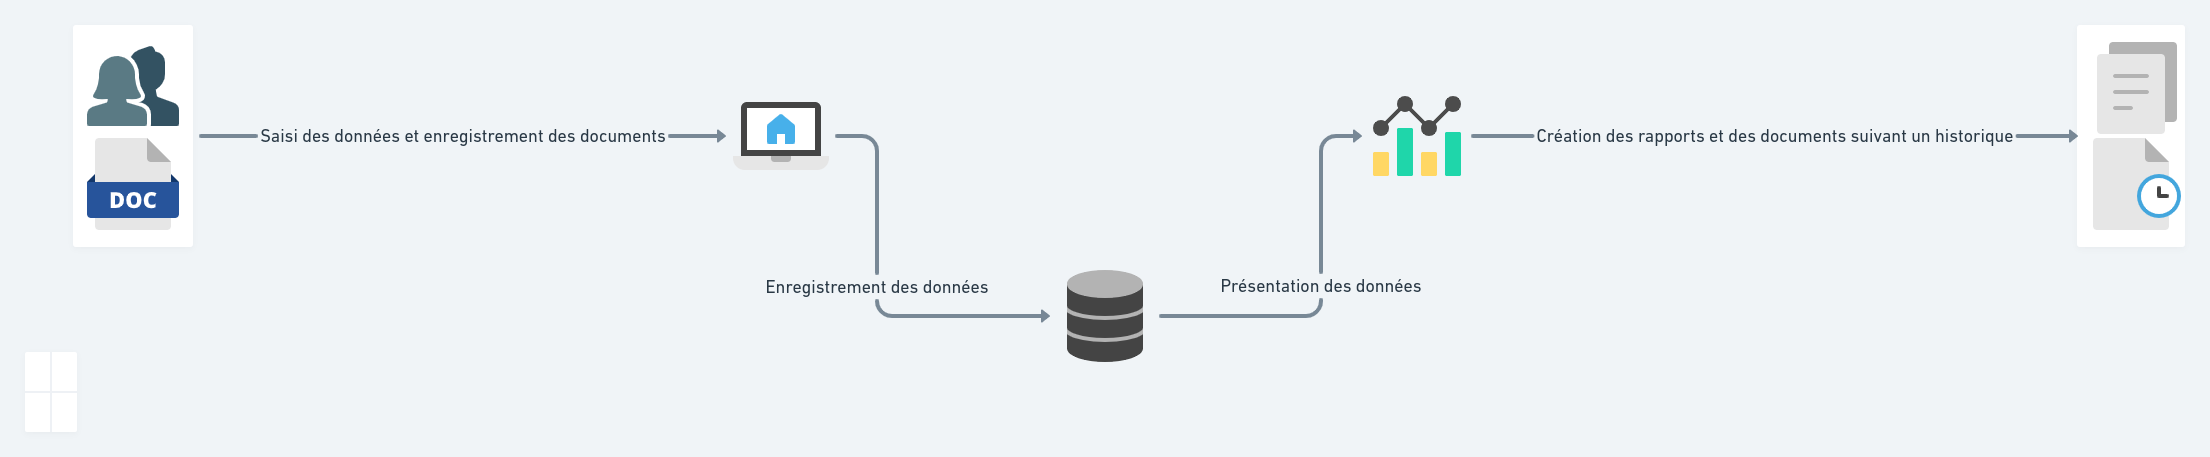
\includegraphics[scale=0.2]{pre-descip-projet.png}}
        \caption{Description préliminaire du projet}
    \end{center}
\end{figure}
\subsection{Étude de l’existant}

Après la recherche et des exemples similaire à notre projet, on a
trouvé une diversité des sites web et des applications dédiées à la gestion et
au suivi.
À titre d'exemple on peut considérer l'application \textbf{\large Ecan}:

Généralement, les applications similaires sont des applications qui
aide à la gestion des données et des ressources, et la prise des décisions.
L’application \emph{Environnement Canterbury (ECan)} fait partie du
gouvernement local de la région de Canterbury en Nouvelle-Zélande. Ils ont
utilisé la plate-forme \emph{Power
    (PowerApps, Microsoft Flow et Power BI)} pour gérer et rendre compte
efficacement des projets d'eau douce et de ressources naturelles.

D’après l'article intitulé Environnement Canterbury accélère le suivi
des
résultats avec \emph{la Power Platform} :
« Environnement Canterbury travaille en partenariat avec les communautés
de
Canterbury pour promouvoir la gestion durable des ressources
naturelles. Cela
implique l'utilisation de méthodes innovantes, rentables et
techniquement
excellentes, et garantit que la prise de décision est basée sur des
informations
de la plus haute qualité. Ils travaillent sur des programmes de
résultats
environnementaux à long terme qui consistent en plusieurs étapes et
projets
connexes. ECan avait besoin d'une solution abordable qui offrirait une
plus
grande cohérence entre les projets, des niveaux de visibilité plus
élevés et un
accès plus rapide aux données ».
\begin{figure}[H]
    \begin{center}
        \fbox{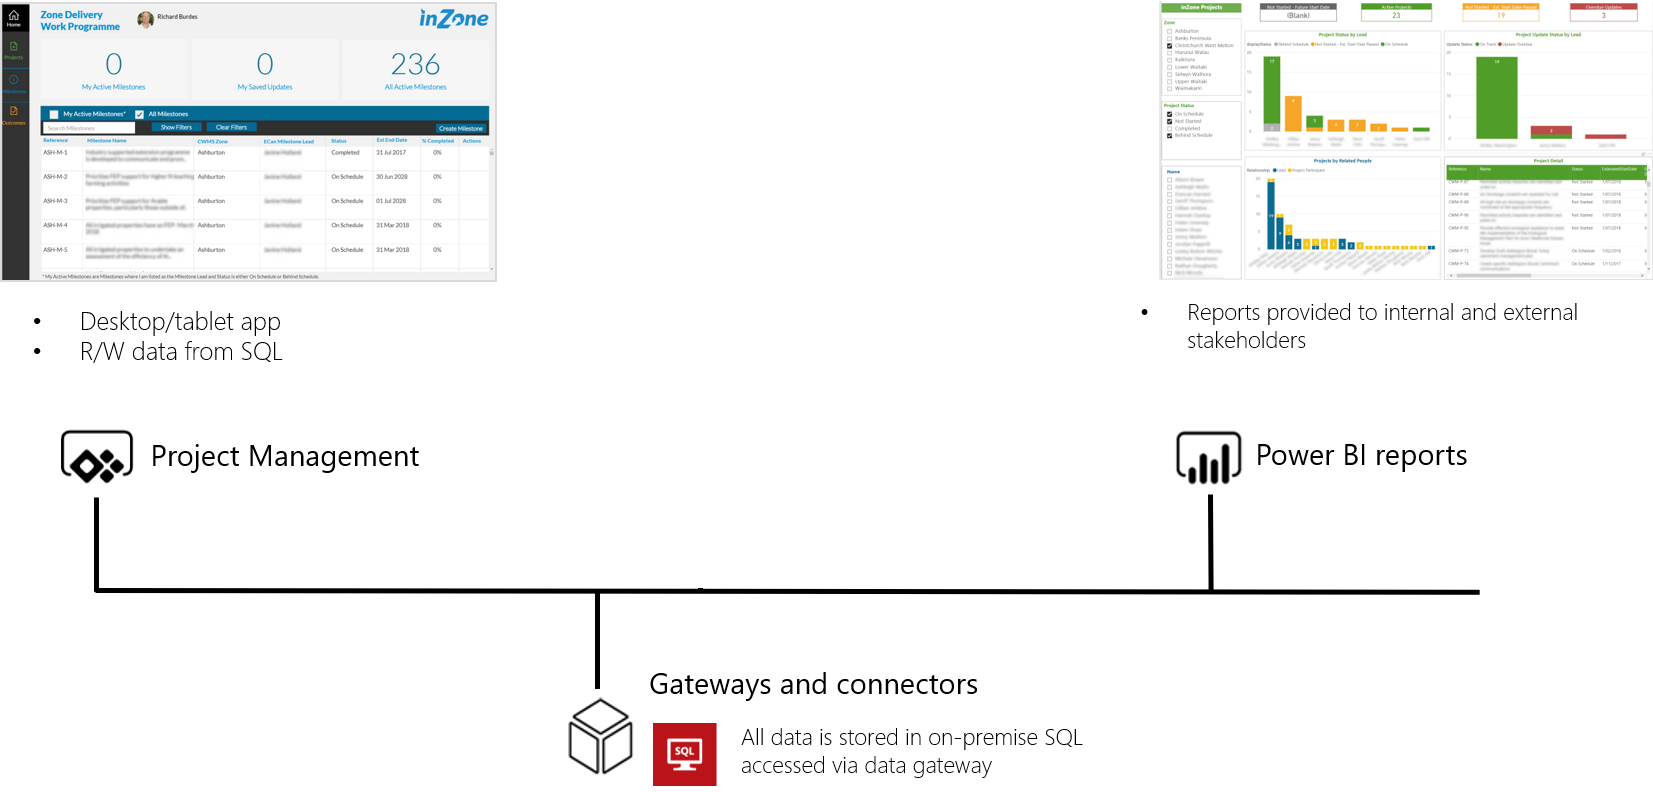
\includegraphics[scale=0.32]{example.png}}
        \caption{Exemple de Environnement Canterbury (ECan)}
    \end{center}
\end{figure}
\newpage
\section{Spécification des besoins}

\subsection{Spécification des acteurs}
Vu que les informations gérées par cette application sont des informations confidentielles de l'état, l'application va avoir en général un seul acteur:
L'administrateur est la personne chargée de charger les informations des différentes communes et de gérer leurs données, préparées par les différentes communes du Maroc.
\subsection{Besoins fonctionnels}
\begin{itemize}
    \item[•] Gestion des délégants et des délégataires: L'administrateur doit avoir
          une section où il pourra gérer les délégants et les délégataires.
    \item[•] Gestion des contrats: Il doit avoir également la possibilité de gérer les contrats signés. En addition, il peut suivre les avenants et les révisions de chaque contrat. Ainsi que le statuts de chaque avenant ou révision.
    \item[•] Gestion des Avancements: L'application doit permettre de gérer les avancements semestriels des contrats. Aussi, consulter et suivre les changements apportés à chaque période.
    \item[•] Présentation des tableaux de bord: L'application doit présenter des données historiées de chaque contrat permettant de bien estimer la qualité de service en question et prendre les bonnes décisions.
    \item[•] Sauvegarde des fichiers sur un serveur WEB, et de sauvegarder en base de données le chemin de celui-ci. Généralement, cette solution est assez efficace, assez simple à mettre en œuvre.
\end{itemize}
\subsection{Les besoins non fonctionnels}
Les besoins fonctionnels sont basiques pour un fonctionnement
correcte et une réponse fiable aux besoins des utilisateurs, mais il y a d'autres besoins qui tendent à améliorer la performance et la qualité de
l'application pour une utilisation plus adéquate.
\begin{itemize}
    \item[•] Fiabilité de la plateforme: L’application doit
          fonctionner sans erreur.
    \item[•] Ergonomie, souplesse et confort d’utilisation: Pour
          faciliter l’utilisation, notre plateforme doit offrir une interface unifiée,
          conviviale et ergonomique.
    \item[•] Gain de temps: L'application doit optimiser les
          traitements pour avoir un temps de réponse minimale.
    \item[•] Maintenabilité et sociabilité: La source de l'application doit être compréhensible
          afin d’assurer son état évolutif et extensible par rapport aux besoins des utilisateurs. En outre, l’expérience des utilisateurs doit être meilleurs.
    \item[•] Sécurité: Notre plateforme doit  être très authentique en ce qui concerne les informations confidentielles des communes.
\end{itemize}
\section{Analyse fonctionnelle}
Suivant à ce qui précède et d’après l’ensemble des documents communiqués par mes encadrants, j’ai essayé de créer une décomposition hiérarchique des fonctionnalités du projet.
\begin{figure}[H]
    \begin{center}
        \fbox{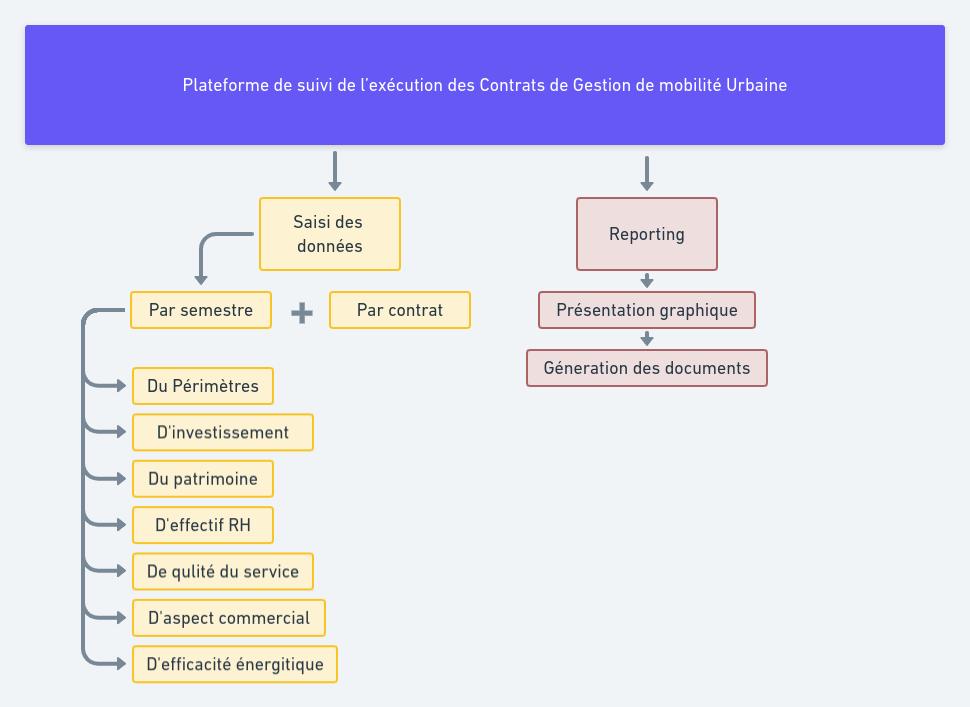
\includegraphics[scale=0.5]{WBS KPI.png}}
        \caption{Décomposition fonctionnelle du projet}
    \end{center}
\end{figure}
Ainsi, J'ai divisé le projet en deux parties fondamentales. En plus, on peut voir clairement les grandes fonctionnalités demandées dans cette application. Par conséquent, l'application peut être divisée en deux partie: partie saisi et partie reporting.
\begin{itemize}
    \item[•] La partie saisi est la partie dans laquelle l'administrateur peut ajouter des délégants et des délégataires. En conséquences, il peut définir un contrat. Par ailleurs, le contrat définit peut avoir des mises à jour semestriels des informations qui le concerne.
    \item[•] La partie reporting est la partie qui concerne les tableaux de bords de l’application. Il doit bien présenter les informations saisîtes. En plus, il est préférables d'avoir la possibilité de générer des documents contenants les informations saisîtes.
\end{itemize}
\section{Analyse technique}
La solution que je propose est une solution basée sur les données.
Autrement dite, elle permet à son utilisateur d'interagir avec plusieurs
informations. En outre, elle représente une solution spécialisée pour
l'acquisition, la gestion et la présentation d'informations. Ainsi, le groupe du projet à proposer l'ensemble des outils suivants:
\begin{figure}[H]
    \begin{center}
        \fbox{
\includegraphics[scale=0.41]{outilsDB.png}}
        \caption{Base de donnée SQL SERVER}
    \end{center}
\end{figure}
Microsoft SQL Server est un système de gestion
de base de données relationnelle développé
par Microsoft. En tant que serveur de base de
données, il s'agit d'un produit logiciel dont la
fonction principale est de stocker et de
récupérer des données à la demande d'autres
applications logicielles, qui peuvent
s'exécuter sur le même ordinateur ou sur un
autre ordinateur via un réseau.
\begin{figure}[H]
    \begin{center}
        \fbox{
\includegraphics[scale=0.41]{outilsDEV.png}}
        \caption{Microsoft Power Apps}
    \end{center}
\end{figure}
Power Apps est un service permettant de créer
et d'utiliser des applications professionnelles
personnalisées qui se connectent à vos
données et fonctionnent sur le Web et les
appareils mobiles - sans le temps et les frais
de développement de logiciels personnalisés.
\begin{figure}[H]
    \begin{center}
        \fbox{
\includegraphics[scale=1.1]{outilsREP.png}}
        \caption{Microsft Power BI}
    \end{center}
\end{figure}
Power BI est un service d'analyse
commerciale de Microsoft. Il vise à fournir des
visualisations interactives et des capacités de
business intelligence avec une interface
suffisamment simple pour que les utilisateurs
finaux puissent créer leurs propres rapports et
tableaux de bord. Il fait partie de la plateforme
Microsoft Power.

Suite à cette proposition le consultant technique a approuver ces choix. Ainsi la décision est prise d'utiliser ces technologies Microsoft afin de réaliser une application Low-Code pour la gestion des contrats de gestion déléguée du transport urbain par autobus.
\section{Planification et démarche de travail}
\subsection{Plan de travail prévu}
Pour la bonne organisation des étapes du projet, j'ai proposé premièrement le plan suivant pour la réalisation de la plateforme demandée:
\begin{figure}[H]
    \begin{center}
        \fbox{\includegraphics[scale=0.3]{GanttPrévu.png}}
        \caption{Plan de travail prévu du projet}
    \end{center}
\end{figure}
\subsection{Définition des Livrables}
À la fin de chaque étape de la réalisation
(section dans le diagramme de Gantt si-dessus),
il est exigé d'avoir un livrable.
Les livrables que nous proposons sont les suivants:
\begin{table}[H]
    \begin{center}
        \begin{tabularx}{17.5cm}{|p{2cm}|X|}
            \hline
            \textbf{Étape} & \textbf{Livrable}                                                                                                                                                                  \\
            \hline
            Analyse        & Document de spécification décrivant le besoin, les fonctionnalités de la solution à implémenter, les technologies à utiliser, et toutes les contraints à respecter dans le projet. \\
            \hline
            Conception     & Document de conception qui donne une idée clair et global sur le projet.                                                                                                           \\
            \hline
            Réalisation    & Plateforme de suivi de l’exécution des contrats de gestion de mobilité urbaine.                                                                                                    \\
            \hline
        \end{tabularx}
        \caption{Livrables prévus de projet}
    \end{center}
\end{table}
\subsection{Les acteurs du projet}
\begin{itemize}
    \item[•] \textbf{L’équipe du travail:} La tâche de la conception et de développement de l’application est assigné à moi.
    \item[•] \textbf{Le product owner:} Qui est ici la \textbf{DGCT} représenté par M.\textbf{LABIZ} Ibrahim. Il tient le rôle de définir les fonctionnalités et de s’assurer du bon fonctionnement du projet.
    \item[•] \textbf{Le SCRUM master:} Mon encadrante, Mme.\textbf{TAHLAOUI} Insaf a tenu ce rôle, en veillant sur la réalisation du projet.
\end{itemize}
\subsection{Les sprints du projet}
Pour le bon déroulement du projet, le travail sera découpé en sprint. Ces sprints sont établi à l’aide du product backLog tout en respectant la priorité des différents modules. À la fin de chaque sprint, on aura un livrable qui sera examiné par le Product Owner afin de planifier les modifications et les évolutions à effectuer dans le sprint suivant. La planification du projet selon les sprints et comme suit :
\begin{table}[H]
    \begin{center}
        \begin{tabularx}{17.5cm}{|p{2cm}|p{2cm}|X|}
            \hline
            \textbf{Numéro} & \textbf{Durée} & \textbf{Description}                                                                            \\
            \hline
            1               & 2 semaines     & Réalisation et connexion à la base de donnée.                                                   \\
            \hline
            2               & 2 semaines     & Création de la partie gestion des contrats et d'un référence des délégants et des délégataires. \\
            \hline
            3               & 2 semaines     & Création de la partie suivis des contrats.                                                      \\
            \hline
            4               & 2 semaines     & Réalisation des tableaux de bords demandés.                                                     \\
            \hline
        \end{tabularx}
        \caption{Les Sprints du projet}
    \end{center}
\end{table}
\subsection{Mode de travail}
Afin de réaliser le projet, on doit définir un mode de travail convenable. Le mode de
travail que je propose est le mode agile en utilisant SCRUM. Puisque je travaille
dans un environnement où je garde un contact continue avec le Product Owner. En
plus, je cherche à avoir une communication efficace avec le client pour le
satisfaire en lui livrant fréquemment un état d'avancement tangible.
D'ailleurs, le temps est un facteur important dans ce projet. De ce fait, il faut sentir
l’avancement quotidienne du projet. En addition, il faut faire attention continue à
l’excellence technique, à une meilleure conception et produire uniquement ce qui est
nécessaire dans les meilleurs délais. Pour ce faire j'ai utilisé la plateforme Trello. Ainsi, on présente le tableau suivant basée sur le modèle kanban pour l'organisation des tâches et des livrables:
\begin{figure}[H]
    \begin{center}
        \fbox{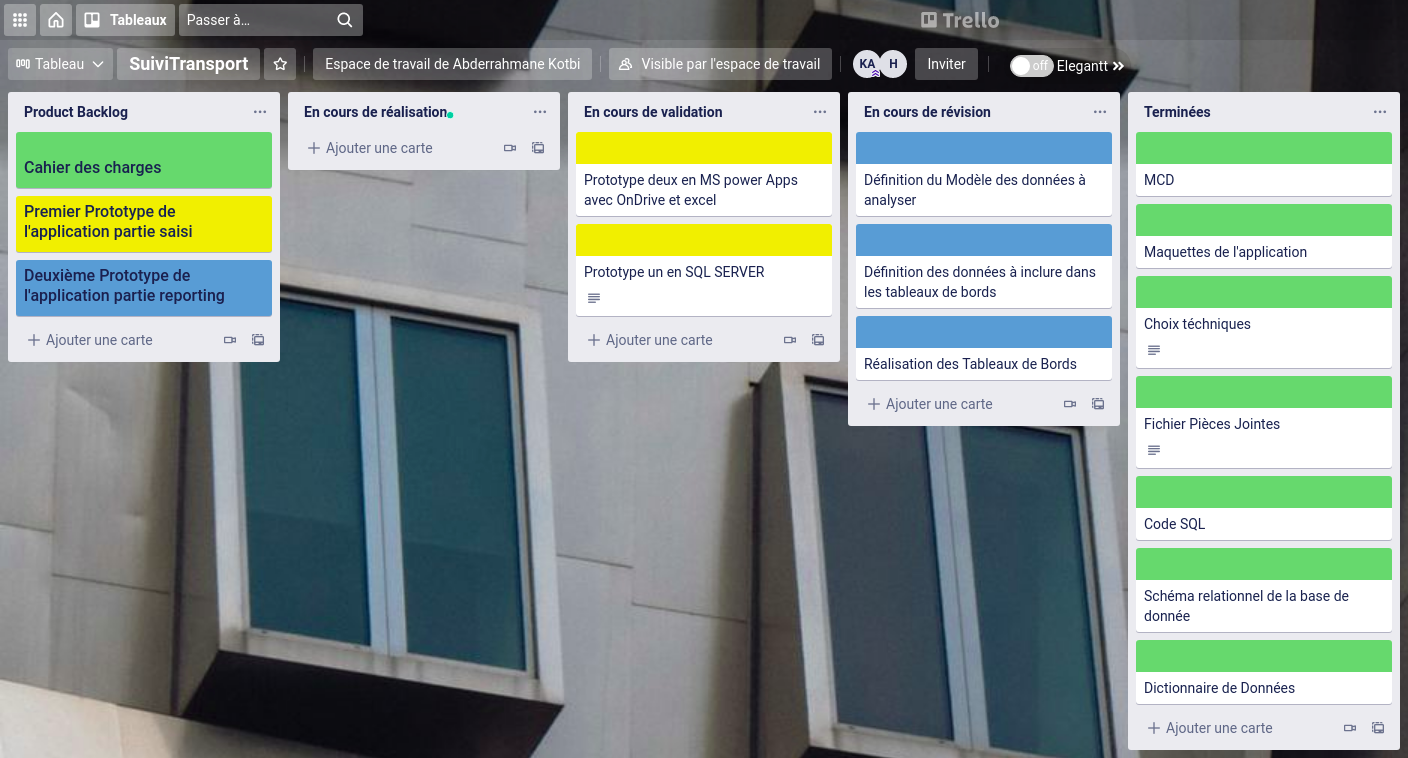
\includegraphics[scale=0.37]{trello.png}}
        \caption{Modèle Kanban du projet}
    \end{center}
\end{figure}
\section{Récapitulatif}
Dans ce chapitre, j'ai déterminé les acteurs principaux dans ce projet ainsi que leur
besoin. L'étude élaborée serai ma base de travail par la suite, à
savoir: la conception et la réalisation de notre projet. Dans le chapitre suivant je vais
exposer ma vue conceptuelle vis-à-vis au projet.
\begin{figure}[H]
    \begin{center}
        \fbox{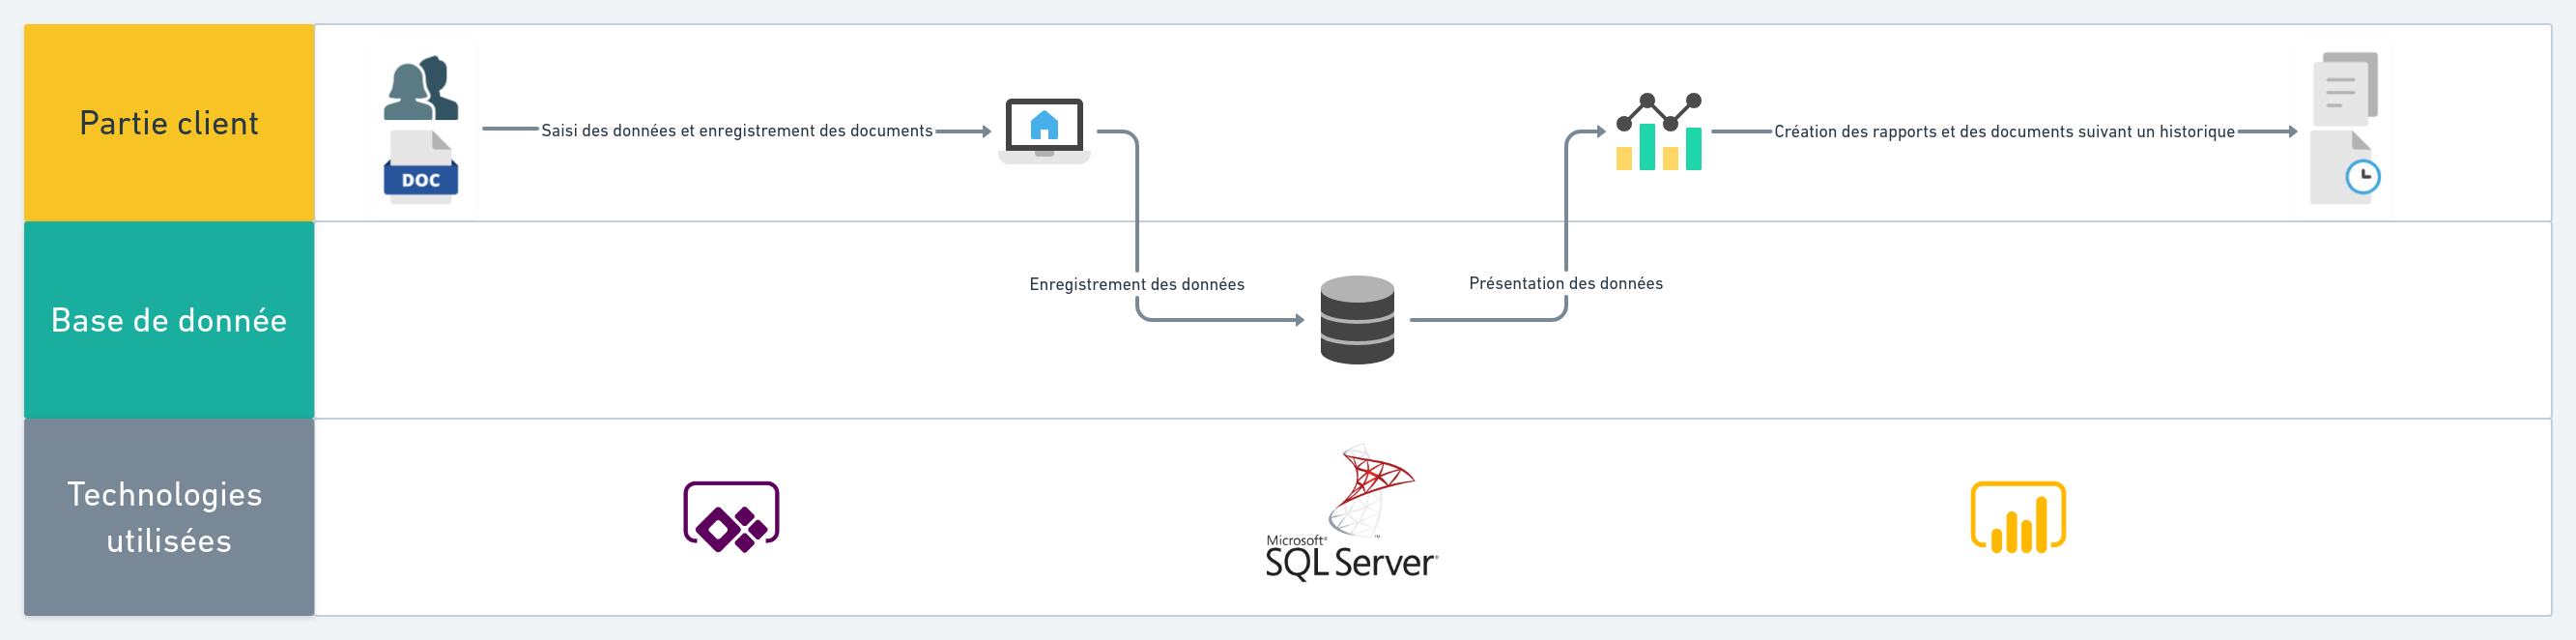
\includegraphics[scale=0.19]{KDI.png}}
        \caption{Description générale du projet}
    \end{center}
\end{figure}
